\chapter{前後端傳輸}
\section{技術介紹}
前後端的傳輸主要使用UDP Socket來做傳輸,主要功能如下:
\begin{itemize}
\item 將手機後相機影像傳送至伺服器,交由神經網路模組辨識手勢。
\item 多人遊玩 - 玩家之間的遊戲資料傳遞。 
若使用者有中靶,傳遞飛鏢的Pose(Translation \& Quaternion)參數至伺服器,在將這些資料傳遞至其他使用者讓其他使用者能看到彼此發射的飛鏢。
\end{itemize}
\subsection{傳輸流程說明}
\begin{figure}[h]
    \centering	
    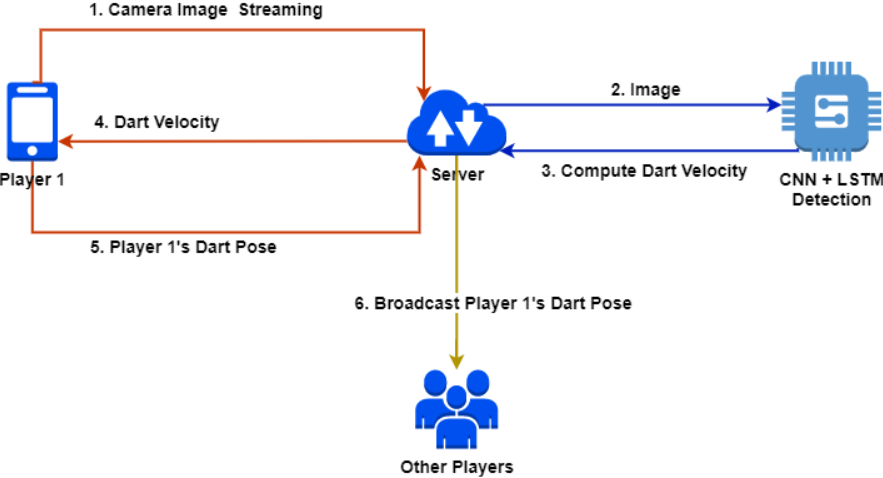
\includegraphics[width=\textwidth]{flow.png}
    \caption{流程圖}
    \label{fig:flow}
\end{figure}
\begin{enumerate}
\item 手機後相機影像擷取,傳輸至伺服器。
\item 伺服器解壓影像,將影像傳送至神經網路模組。
\item 神經網路模組辨識飛鏢速度 。
\item 飛鏢速度由伺服器端傳送至手機端。
\item 若玩家中靶,則將飛鏢之位置(Pose)傳送至伺服器。
\item 伺服器傳送中靶位置給其他使用者。
\end{enumerate}

影像以及遊戲資料個別使用一個Socket,目的是將資料分流,另外也能夠在伺服器端做multi-process的處裡,加快處裡速度。
\subsection{手機端實作}
\subsubsection{手機後相機影像的擷取}
1. 在onDrawFrame()裡,在camera preview image render到 GL surface之後,將GL的surfaceView儲存到buffer,轉換為Bitmap。

2. 每個pixel需儲存R,G,B,A這四個資料,因此 buffer allocate memory = surfaceView’s width * height * 4 bytes。

3. 在create完buffer後,需呼叫rewind(),將buffer的position設為0,將讀取的資料位置從0開始。\href{可於此處}{https://stevenitlife.blogspot.com/2015/01/java-nio-socket-bytebuffer-method.html} 了解相關buffer使用方法。

\begin{lstlisting}[language=Java, caption=手機後相機影像擷取]
// Create buffer: allocate memory( 1 pixel = 4 bytes(R, G, B, A))
ByteBuffer bf = ByteBuffer.allocateDirect(surfaceView.getWidth() * surfaceView.getHeight() * 4);
// Using nativeOrder to store in buffer (other option: Big Endian / Little Endian)
bf.order(ByteOrder.nativeOrder());

// Camera view to buffer
GLES10.glReadPixels(0, 0, surfaceView.getWidth(), surfaceView.getHeight(),
        GLES30.GL_RGBA, GLES30.GL_UNSIGNED_BYTE, bf);
// Create bitmap
Bitmap bmp = Bitmap.createBitmap(surfaceView.getWidth(), surfaceView.getHeight(), Bitmap.Config.ARGB_8888);
bf.rewind();
// Copy buffer data to bitmap
bmp.copyPixelsFromBuffer(bf);

conn.mBackgroundHandler.post(conn.new SendImageData(bmp));
\end{lstlisting}

\subsubsection{傳輸影像至伺服器端}
1. Android的操作,只要超過5秒沒回應(或OnCreate()超過10秒),程式就會被當作無回應,而系統會丟出ANR(Application No Response Exception)。所以,比較耗時費工的動作,都應該考慮用背景作業的方式來完成(另外這些background thread不能包含UI的處理),此處傳輸即用Background Thread做處理。

2. 使用UDP socket傳輸,和TCP不同的是,每次UDP送出的封包都需指定送出的對象(connectionless protocol),不須事先建立連線,且沒有重送封包的機制,因此我們在此專題需要即時上的應用時,選用此技術。

3. 在傳輸Bitmap時,需要轉為byteArray,另外,將Bitmap resize 原大小的1/100,目的想將資料傳輸量盡量變小,降低延遲。

\begin{lstlisting}[language=Java, caption=傳輸影像至伺服器端]
public class SendImageData implements Runnable {
        private Bitmap mBitMap;
        private Bitmap resizeBitMap;
        private byte[] data = null;

        public SendImageData(Bitmap bmp) {
            mBitMap = bmp;
            resizeBitMap = Bitmap.createScaledBitmap(mBitMap, mBitMap.getWidth() / 10, mBitMap.getHeight() / 10, true);
        }

        @Override
        public void run() {
            try {
                if (serverAddr == null) {
                    serverAddr = InetAddress.getByName("140.121.196.201");
                }
                if (socket == null) {
                    socket = new DatagramSocket();
                }

                ByteArrayOutputStream byteStream = new ByteArrayOutputStream();
                resizeBitMap.compress(Bitmap.CompressFormat.JPEG, 80, byteStream);
                data = byteStream.toByteArray();
                try {
                    DatagramPacket packet = new DatagramPacket(data, data.length, serverAddr, 5000);
                    Log.i("data length", String.valueOf(data.length));
                    socket.send(packet);
                } catch (Exception e) {
                    System.out.println("Error 1:" + e.toString());
                }
            } catch (Exception e) {
                System.out.println("Error 2:" + e.toString());
                socket.close();
            }
            mBitMap.recycle();
        }
    }
\end{lstlisting}
\subsection{系統延遲實驗}
\subsubsection{實驗說明}
為達良好之遊戲體驗,故衡量玩家從傳輸影像到拿到回傳參數的時間。而為將各個變因獨立衡量,將分析延遲如下圖所示:

\begin{figure}[h]
    \centering	
    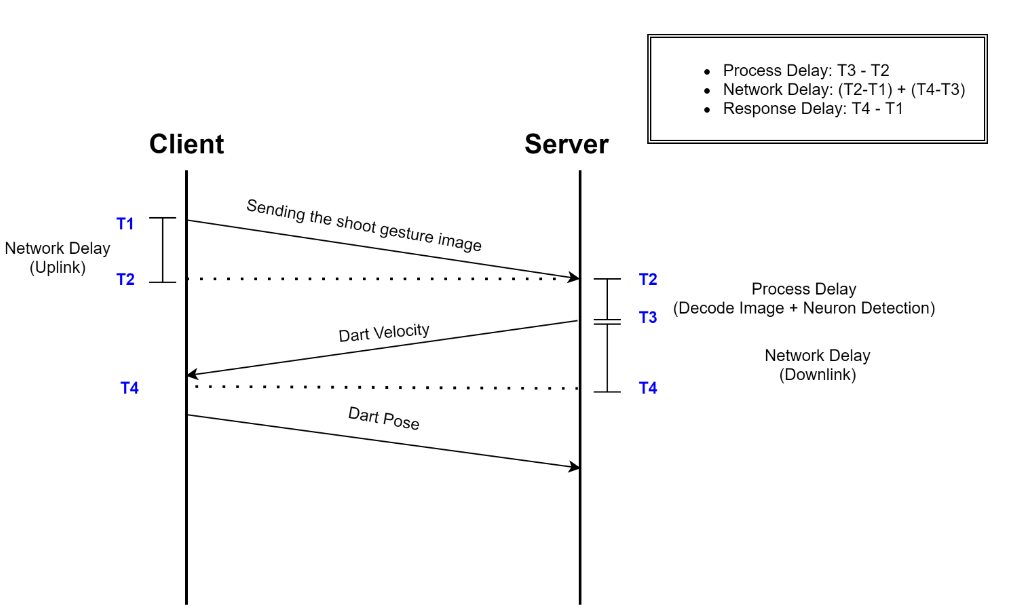
\includegraphics[width=\textwidth]{latency.png}
    \caption{解構響應延遲}
    \label{fig:decomposition of response delay}
\end{figure}

\begin{itemize}
\item Response Delay:
總延遲,玩家由送出手機後相機影像,至拿到飛鏢初速之時間。根據上圖所示,計算方式為T4 - T1。
\item Process Delay:
伺服器端處裡時間,包含影像解碼、神經網路辨識,到送出飛鏢速度的這段時間。根據上圖所示,計算方式為T3 - T2。
\item Network Delay:
網路延遲時間,分為uplink、downlink delay。根據上圖所示,計算方式為(T2-T1) + (T4 - T3)。
\end{itemize}
\subsubsection{系統延遲實驗結果\&分析}
Network Delay主要以ping server來分析,而經過約15次的測試下,平均Network Delay介於40 - 60 ms之間。

Process Delay 則以伺服器接收到影像的時間搓記,與送出封包的時間搓記,來計算其時間差,實驗兩次,每次計算約80 - 100張影像,平均值為7.02 ms 以及7.72ms,Process Delay結果如下圖所示。

\begin{figure}[h]
    \centering	
    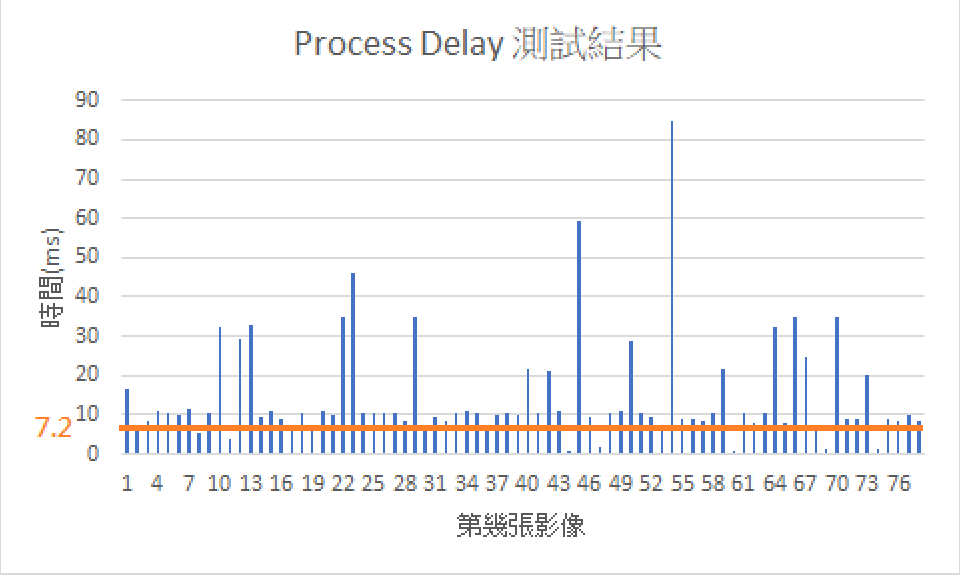
\includegraphics[width=\textwidth]{process_delay.png}
    \caption{實驗一之結果}
    \label{fig:Process delay bar chart}
\end{figure}

結果顯示,Response Delay介於47.02 - 60.72 ms之間,故在發射飛鏢手勢時,不會感到明顯延遲。

